%=====================================================================
\section{Passive circles: where the imposed defects sit}\label{sec:passive}
Without activity the imposed winding produces exactly $2|k|$ defects of the sign of $k$ and nothing else. This section
establishes where they sit, as the reference for everything active.

\paragraph{Data.} Passive references of the main sweep (\texttt{main\_passive}, \texttt{main\_passive\_neg}): one seed
per point, activity 0, 10k warm-up + 30k steps, defects every 50 steps; the same $(\rho,k)$ grid as the active sweep,
$k=\pm1\dots\pm20$, $\rho=0.03$--0.50 (468 runs in total, 278 with $+k$, 190 with $-k$). Earlier validation runs at $R=15$,
$k=\pm1\dots\pm5$ (\texttt{runs/cavityValidation/passive}). Analysis: \texttt{reports/master/scripts/fig\_passive.py}
(frames after the first 20\%; $s=R-r$; table \texttt{reports/master/data/passive\_circles.tsv}).

\begin{figure}[H]\centering
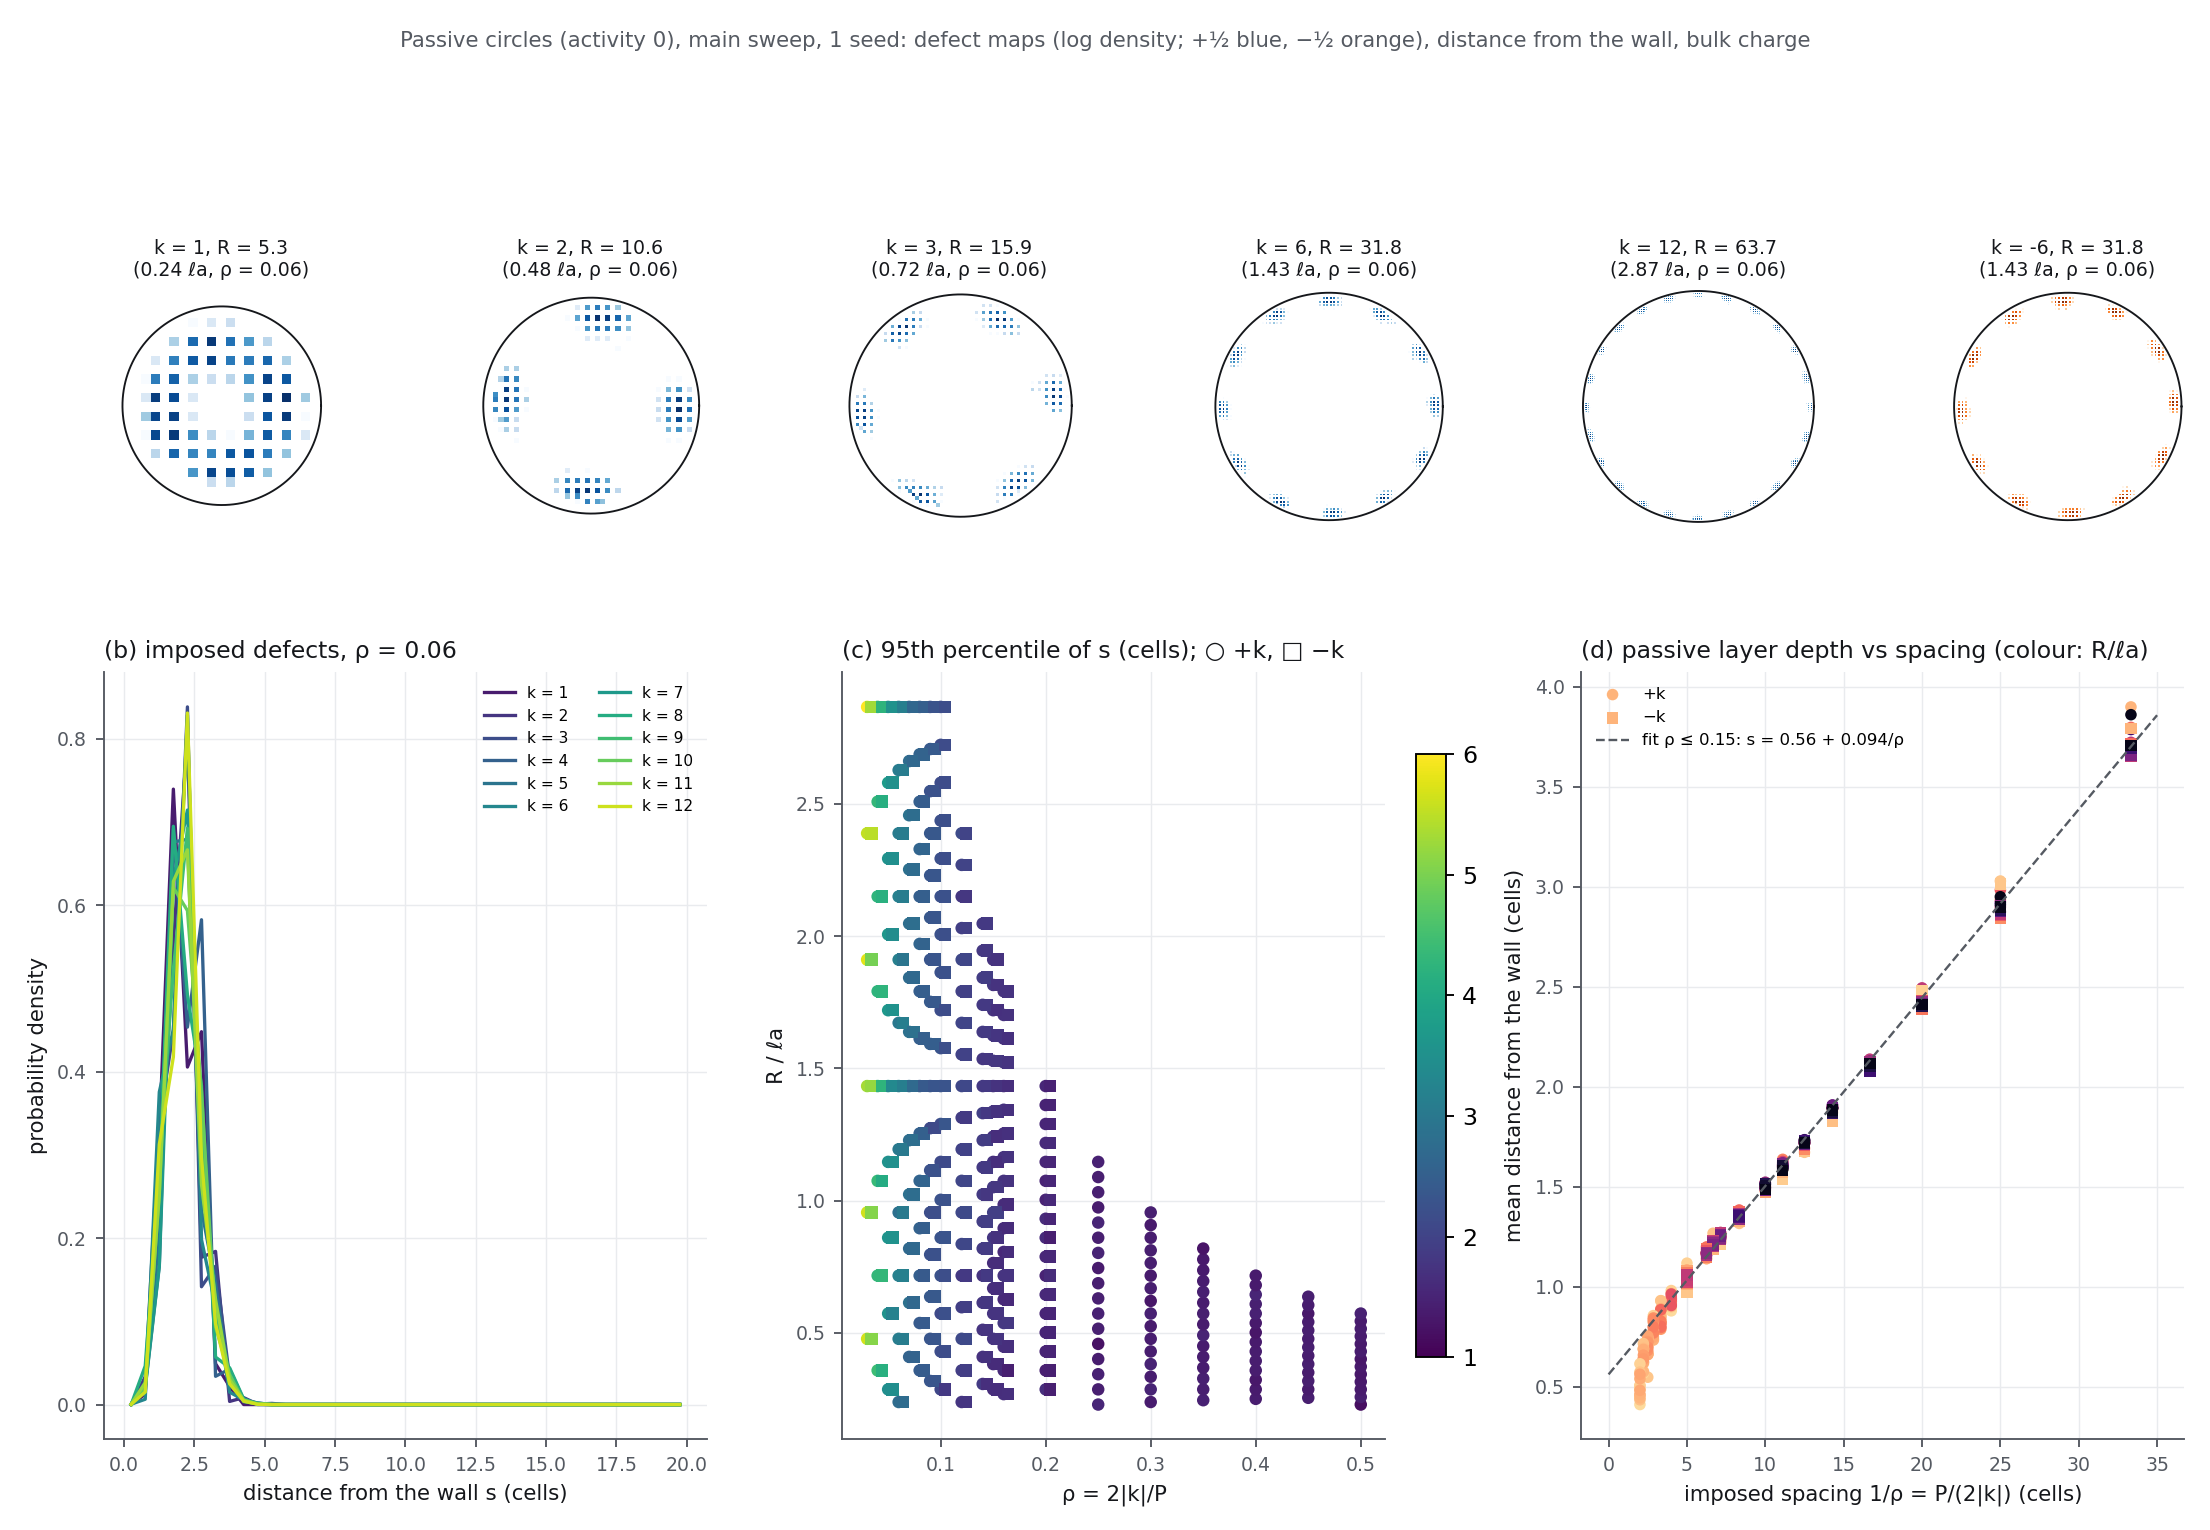
\includegraphics[width=\textwidth]{passive_circles.png}
\caption{Passive circles. (a) Time-averaged defect density (log scale, $+\half$ blue, $-\half$ orange) for $k=1,2,3,6,12$
at $\rho=0.06$ and for $k=-6$: the defects sit on $2|k|$ fixed sites just inside the wall. (b) Distribution of the distance
$s$ from the wall of the imposed defects, $k=1\dots12$ at $\rho=0.06$: the same narrow peak at $s\approx2$ cells for every
$k$. (c) 95th percentile of $s$ over the sweep ($\circ$ $+k$, $\square$ $-k$): it depends on $\rho$ only. (d) Mean $s$
against the imposed spacing $1/\rho$, all 468 runs (colour $R/\la$): a single line,
$\langle s\rangle\approx0.56+0.094/\rho$ cells for $\rho\le0.15$, identical for both signs.}\label{fig:passive}
\end{figure}

\paragraph{Results.}
\begin{itemize}
  \item \textbf{Every imposed defect is present, and nothing else.} $N_\pm$ per frame equals $2|k|$ of the imposed sign
        and 0 of the other sign to two decimals in every run with $\rho\le0.15$; the median fraction of frames with exactly
        this configuration is 0.994. At $\rho=0.20$ it drops to 0.76--0.90, the anchoring resolution limit
        (Sec.~\ref{sec:resolution}).
  \item \textbf{They sit on fixed sites} at equal spacing along the wall (Fig.~\ref{fig:passive}a), $2|k|$ of them;
        the time-averaged maps show compact spots, so the defects do not move along the wall (their apparent speed,
        0.3 cells per time unit, is the detection jitter of the cell-based tracker; Fig.~\ref{fig:prof-circ}).
  \item \textbf{Their depth is set by the imposed spacing only} (Fig.~\ref{fig:passive}d): the mean distance from the wall
        grows linearly with $1/\rho$, from $\approx1$ cell at $\rho=0.2$ (spacing 5) to 3.9 cells at $\rho=0.03$ (spacing 33),
        independent of $R$ and of the sign of $k$. A defect sits deeper when its neighbours along the wall are farther
        away, as expected for a director field that relaxes the imposed winding over a distance comparable with the spacing.
  \item This explains two observations that looked like exceptions earlier. In the $R=15$ validation run, $k=1$ placed its
        two $+\half$ at $r\approx9$--10, i.e.\ $s\approx5$--6: the spacing is 47 cells, where the line predicts 5.0. In the
        passive fixed-radius scan ($R=31.8$), $k=2$ sat at $s\approx5.7$ (spacing 50, predicted 5.3), which was read as
        ``no layer''; across that scan ($\rho=0.02$--0.10) the passive layer shrank from 8.3 to 2.3 cells with $k$ for the same
        reason. A passive ``layer width'' is therefore not a good edge for the active bulk (Sec.~\ref{sec:edge}).
  \item \textbf{Bulk charge 0.} The charge enclosed inside the defect ring is zero in every frame: all charge is in the
        wall layer. A fixed cut at 5 cells from the wall wrongly counts some wall defects as bulk at $\rho\le0.04$, where
        the layer is deeper than 5 cells (up to $|q|\approx0.95$ at $\rho=0.03$, $R=2.9\,\la$); this is a cut artefact, not
        a bulk charge.
  \item \textbf{Mirror symmetry is exact.} With $-k$ the same number of $-\half$ appears at the same depths
        (Fig.~\ref{fig:passive}d, squares); at $R=15$, $k=-2,-3$ reproduce $k=2,3$ (alignment 0.99, $Q(R-1)=-2.00/-3.00$).
        Any asymmetry between the signs in active runs is therefore an active effect.
  \item \textbf{Anchoring quality.} At $R=15$ the wall director follows the imposed winding with alignment 0.96--0.99;
        \texttt{customAnch} = 0 and 1 give identical results.
\end{itemize}
